% Functional-Requirement Table Design
%
% Oberhalb und unterhalb des Zeilen Contents muss noch irgendwie Platzeingefügt werden
\newcounter{linkcount}
\newcounter{linktotal}

\newcommand{\countLinks}[1]{%
    \setcounter{linkcount}{0}%
    \setcounter{linktotal}{0}%
    \renewcommand*{\do}[1]{\stepcounter{linktotal}}%
    \docsvlist{#1}%
}

\newcommand{\createHyperlinks}[1]{%
    \ifthenelse{\equal{#1}{-}}%
    {-}%
    {%
        \countLinks{#1}%
        \renewcommand*{\do}[1]{%
            \stepcounter{linkcount}%
            \hyperlink{FA##1}{FA##1}%
            \ifnum\value{linkcount}<\value{linktotal}%
            ,\ %
            \fi%
        }%
        \docsvlist{#1}%
    }%
}

\newcommand{\reqTable}[4]{
        {\rowcolors{2}{gray!50!white!20}{gray!40!white!10}
    \phantomsection\hypertarget{FA#1}{}
    \begin{tabular}{ p{3cm} p{10.2cm} }
        \rowcolor{darkgray}\textcolor{white}{\textbf{ID:}} & \textcolor{white}{\textbf{FA#1}} \\
        Titel: & #2 \\
        Beschreibung: & #3 \\
        Abhängigkeit: & \createHyperlinks{#4} \\
    \end{tabular}
    }
}

\newcommand{\createHyperlinksNFA}[1]{%
    \ifthenelse{\equal{#1}{-}}%
    {-}%
    {%
        \countLinks{#1}%
        \renewcommand*{\do}[1]{%
            \stepcounter{linkcount}%
            \hyperlink{NFA##1}{NFA##1}%
            \ifnum\value{linkcount}<\value{linktotal}%
            ,\ %
            \fi%
        }%
        \docsvlist{#1}%
    }%
}
\chapter{Evaluationsframework}\label{ch:evaluationsframework}

Dieses Kapitel stellt das Evaluationsframework vor, das die in Kapitel~\ref{ch:klassifizierungsalgorithmus-(design-und-implementierung)} entwickelte Klassifizierungspipeline nutzt, um verschiedene \acp{LLM} anhand gelabelter Testdaten systematisch, reproduzierbar und transparent zu vergleichen. Leitendes Gestaltungsprinzip ist die Entkopplung: Modelle und Klassifizierungsalgorithmen werden zur Laufzeit konfiguriert und sind dadurch austauschbar. So ermöglicht das Framework einen fairen Vergleich unterschiedlicher Modelle und Verfahren.

\section{Use-Cases und Anforderungen}\label{sec:anforderungen-und-use-cases}

Das Evaluationsframework richtet sich an Forschende und Entwickler, die \acp{LLM} und Klassifizierungsalgorithmen für die Identifikation \ac{DSGVO}-kritischer \ac{BPMN}-Aktivitäten auswerten und miteinander vergleichen möchten. Es bietet eine einheitliche Ausführungs- und Auswertungsumgebung mit klar definierten Schnittstellen und standardisierten Berichten. In diesem Kapitel werden die Use-Cases udn Anforderungen des Evaluationsframeworks beschrieben.

\subsection*{Use-Cases}

Die wichtigsten Anwendungsfälle des Evaluationsframeworks sind:

\begin{itemize}
    \item \textbf{Benchmarking von LLMs.} Systematischer Vergleich mehrerer \acp{LLM} auf denselben Datensätzen, mit identischem Algorithmus und identischen Parametern.
    \item \textbf{A/B-Vergleich von Algorithmen.} Gegenüberstellung verschiedener Klassifizierungspipelines, mit z.B.\ alternativen Prompts oder anderem Preprocessing, über eine standardisierte HTTP-Schnittstelle, die in Kapitel~\ref{sec:api-design} definiert ist.
    \item \textbf{Explorative Analyse.} Detaillierte Einsicht pro Modell und Testfall (inklusive Begründungen und Visualisierungen), um Fehlklassifikationen gezielt zu untersuchen.
    \item \textbf{Berichterstellung.} Die Ergebnisse lassen sich als JSON oder Markdown exportieren und später wieder importieren, um sie erneut untersuchen zu können. Sie eignen sich zudem für die Publikation. Die Diagramme werden automatisch erzeugt und stehen ebenfalls zum Download bereit.
\end{itemize}

In dieser Arbeit werden keine A/B-Vergleiche unterschiedlicher Klassifizierungsalgorithmen durchgeführt, sondern lediglich verschiedene \acp{LLM} mit demselben Algorithmus verglichen. Das Framework ist jedoch so konzipiert, dass dies in zukünftigen Arbeiten möglich ist.

\subsection*{Funktionale Anforderungen}

In der folgenden Tabelle sind die funktionalen Anforderungen an das Evaluationsframework aufgelistet, die notwendig sind um Use-Cases zu erfüllen:

\begin{center}
    \reqTable{01}
    {Nutzen gelabelter Testdatensätze}
    {Das Framework kann die gelabelten Testdatensätze benutzten, die mit dem Labeling-Tool aus \ref{sec:labeling-tool} erstellt worden sind.}
    {}
\end{center}

\begin{center}
    \reqTable{02}
    {Vergleichbarkeit von Modellen und Algorithmen}
    {Das Framework erlaubt den direkten Vergleich verschiedener \acp{LLM} sowie unterschiedlicher Klassifizierungsalgorithmen anhand gelabelter Testdaten. Die Anbindung an Klassifizierungsalgorithmen erfolgt über die in Kapitel~\ref{sec:api-design} definierte, standardisierte HTTP-Schnitstelle.}
    {01}
\end{center}

\begin{center}
    \reqTable{03}
    {Deklarative Konfiguration}
    {Ein Evaluationslauf ist vollständig über eine YAML-Datei konfigurierbar. Dazu zöhlen Modelle, Klassifizierungsendpunkte, Testdatensätze, Seed. Experimente werden dadurch portabel und wiederholbar.}
    {02}
\end{center}

\begin{center}
    \reqTable{04}
    {Detaillierte Ergebnisaufbereitung}
    {
    Das Framework gibt Ergebnisse auf zwei Ebenen aus.
    \begin{enumerate}
        \item Pro Testfall und pro Modell: Status (\enquote{bestanden}/\enquote{nicht bestanden}), klassifizierte Elemente mit Begründungen, \ac{TP}/\ac{FP}/\ac{FN}/\ac{TN} und eine Visualisierung der Klassifikation im \ac{BPMN}-Prozess.
        \item Pro Modell als Summe über alle Testfälle: Accuracy, Precision, Recall, F1-Score und die Konfusionsmatrix.
    \end{enumerate}
    Zusätzlich protokolliert das Framework Metadaten der Evaluation, z.\,B. Endpunkt, verwendete Modelle und den Seed.
    }
    {02}
\end{center}

\begin{center}
    \reqTable{05}
    {Frontend}
    {Für eine einfache Bedienung und Ansicht der Ergebnisse bietet das Evaluationsframework ein Frontend an.}
    {02,03,04}
\end{center}

\begin{center}
    \reqTable{06}
    {Visualisierung und Berichte der Gesamtresultate}
    {Kennzahlen werden als Side-by-Side-Diagramme und tabellarisch dargestellt. Zusätzlich stehen Export/Import der Ergebnisse als JSON sowie ein Markdown-Report zur Verfügung.}
    {05}
\end{center}
\section{Architektur und Komponenten}\label{sec:architektur-und-komponenten}

\begin{itemize}
    \item Diagramm zur Architektur erstellen
    \item HTTP-Endpunkt oder CLI zum Starten -> Holen der notwendigen Testdatensätze -> Aufruf der Klassifizierung pro Modell und pro Testcase -> Akkumulieren der Ergebnisse pro Testcase + ggf. frühzeitige Rückgabe des Ergebnisses des Testcase für Live-Ansicht in UI -> Aufarbeiten der akkumulierten Ergebnisse und berechnen wichtiger Metriken
    \item EvaluationController, MultiEvaluationRunner, EvaluationRunner, HttpEvaluator, MetricsAccumulator, ggf. Frontend (Concurrency von MultiEvaluationRunner)
\end{itemize}

\section{Konfiguration einer Evaluierung}\label{sec:konfiguration-einer-evaluierung}

Die funktionale Anforderung \hyperlink{FA03}{FA03} fordert, dass Evaluationsläufe deklarativ konfiguriert werden können. Das Framework unterstützt dies auf zwei Wegen:
Erstens bietet die Weboberfläche, die in \ref{sec:visualisierung-im-frontend} gezeigt wird, die Möglichkeit, Evaluationsläufe interaktiv zu konfigurieren und zu starten.
Zweitens lässt sich eine Evaluierung über eine YAML-Datei beschreiben, die entweder in der Weboberfläche hochgeladen oder per CLI an das Evaluationsframework übergeben wird. Auf diese Weise werden Reproduzierbarkeit und Versionierung der Evaluationsläufe sichergestellt. Listing \ref{lst:evaluation-config} zeigt ein Beispiel für eine solche YAML-Konfiguration. Ein ausführliches JSON-Schema ist im Anhang (Listing \ref{lst:evaluation-config-schema}) zu finden.

Die Evaluierungskonfiguration umfasst die folgenden Bausteine:

\begin{itemize}
    \item \texttt{defaultEvaluationEndpoint} ist der Standardendpunkt für die Klassifizierung. Er wird verwendet, wenn für ein Modell kein eigener Endpunkt angegeben ist. Der Endpunkt muss die in Kapitel \ref{sec:api-design} beschriebene API-Spezifikation erfüllen und kann relativ (gegen die Basis-URL des Evaluationsframeworks) oder absolut (für einen externen Dienst) angegeben werden.
\end{itemize}

\begin{lstlisting}[caption={Beispiel einer Evaluierungskonfiguration in YAML.},label={lst:evaluation-config}]
defaultEvaluationEndpoint: /gdpr/analysis/prompt-engineering
maxConcurrent: 10
repetitions: 3
seed: 42
models:
  - label: Mistral Medium 3.1
    llmProps:
      baseUrl: https://openrouter.ai/api/v1
      modelName: mistralai/mistral-medium-3.1
      apiKey: ${OPEN_ROUTER_API_KEY}
      topP: 1
  - label: Deepseek Chat v3.1
    llmProps:
      baseUrl: https://openrouter.ai/api/v1
      modelName: deepseek/deepseek-chat-v3.1
      apiKey: ${OPEN_ROUTER_API_KEY}
      temperature: 0.1
  - label: GPT oss 120b
    llmProps:
      baseUrl: https://openrouter.ai/api/v1
      modelName: openai/gpt-oss-120b
      apiKey: ${OPEN_ROUTER_API_KEY}
datasets:
  - 2
  - 7
\end{lstlisting}

\begin{itemize}
    \item \texttt{maxConcurrent} gibt die maximale Anzahl parallel auszuführender Testfälle an. So lassen sich beispielsweise \emph{Rate Limits}\footnote{Providerseitige Begrenzungen, etwa \enquote{Requests pro Minute} oder maximale Parallelität. Bei Überschreitung antworten viele Anbieter mit HTTP~429 (\enquote{Too Many Requests}). Zudem drohen strengere Drosselungen.} der angebundenen \acp{LLM} einhalten, um technische Fehler in den Ergebnissen zu vermeiden.
    \item \texttt{repetitions} bestimmt, wie oft die Evaluierung pro Modell wiederholt wird. Die Ergebnisse werden später über alle Wiederholungen aggregiert (siehe Abschnitt~\ref{sec:generierte-resultate}).
    \item \texttt{seed} legt einen Startwert (Seed) für reproduzierbare Evaluationsläufe fest. Auf Basis des Seeds und der Wiederholungsnummer wird für jede Wiederholung deterministisch ein eigener Seed generiert, um unterschiedliche, aber reproduzierbare Ergebnisse zu erzielen. Er wird bei jedem Modell an die \texttt{llmProps} weitergereicht und bei der Kommunikation mit den \acp{LLM} verwendet, sofern diese einen Seed unterstützen.
    \item \texttt{models} enthält die zu evaluierenden Modelle. Jedes Modell besitzt ein \texttt{label} zur Identifikation und optional spezifische \texttt{llmProps}, um die Eigenschaften des verwendeten \acp{LLM} zu definieren. Diese sind identisch zu den in Kapitel \ref{sec:api-design} beschriebenen \texttt{llmProps}.
    \item \texttt{datasets} ist eine Liste von Datensatz-\texttt{ids}, die jeweils eine Menge von Testfällen beinhalten.
\end{itemize}

Wie im Schema in Listing \ref{lst:evaluation-config-schema} gezeigt, kann jedem Modell optional ein eigener\linebreak~\texttt{evaluationEndpoint} zugewiesen werden, der den in \texttt{defaultEvaluation-\linebreak~Endpoint} definierten Standard überschreibt. Dadurch lassen sich unterschiedliche Klassifizierungsalgorithmen oder -versionen gezielt pro Modell vergleichen. Ist kein spezifischer Endpunkt angegeben, greift automatisch der Standardendpunkt.

API-Keys in den \texttt{llmProps} können optional als Umgebungsvariablen referenziert werden, wie im Beispiel in Listing \ref{lst:evaluation-config} gezeigt. So lassen sich sensible Daten sicher handhaben, ohne sie direkt in der Konfigurationsdatei zu speichern. Die Umgebungsvariablen werden zur Laufzeit aufgelöst und müssen daher im Kontext der Anwendung verfügbar sein.
\section{Testdaten}\label{sec:testdaten}

Wie in \hyperlink{FA01}{FA01} beschrieben, kann das Evaluierungsframework die mit dem Labeling-Tool erzeugten Testdatensätze unmittelbar verwenden. Da das Tool die Testdaten in einer Datenbank ablegt, lassen sie sich unkompliziert auslesen und für die Evaluierung heranziehen. In der Konfiguration des Frameworks wird festgelegt, welche Datensätze genutzt werden, wodurch sich die Auswertung gezielt auf einen bestimmten Anwendungsfall zuschneiden lässt. Wie die Konfiguration einer Evaluierung funktioniert, wird im nächsten Kapitel erläutert.
\section{Evaluationsergebnisse}\label{sec:generierte-resultate}

Die im Folgenden beschriebenen Resultate werden während der Evaluierung laufend erzeugt und an das Frontend gestreamt. Anwender können damit sowohl Zwischenstände verfolgen als auch nach Abschluss detaillierte Analysen durchführen.

Für jeden Testfall eines Modells liegen vor: die von der Klassifizierungspipeline klassifizierten Aktivitäten mit optionalen Begründungen, die gelabelten erwarteten Aktivitäten, die Zählwerte für \emph{\ac{TP}}, \emph{\ac{FP}}, \emph{\ac{FN}} und \emph{\ac{TN}} sowie eine Bild-URL zur Visualisierung des \ac{BPMN}-Modells mit hervorgehobenen Aktivitäten. Aus diesen Informationen lässt sich ableiten, ob der Testfall erfolgreich war. Ein Testfall gilt als erfolgreich, wenn die klassifizierten Aktivitäten exakt den erwarteten Aktivitäten entsprechen. Technische Probleme, die während der Klassifizierung auftreten, werden ebenfalls erfasst, z.\,B.\ Parsing-Fehler, ungültiges \ac{BPMN}, Token-Limit-Überschreitungen oder Zeitüberschreitungen.

Auf Modellebene stehen die Gesamtergebnisse über alle Testfälle zur Verfügung. Dazu gehören die aggregierten Kennzahlen \emph{Precision}, \emph{Accuracy}, \emph{Recall} und \emph{F1-Score} sowie eine Konfusionsmatrix mit den Gesamtwerten für \emph{\ac{TP}}, \emph{\ac{FP}}, \emph{\ac{FN}} und \emph{\ac{TN}}. Zusätzlich sind die Anzahlen der korrekt bzw.\ falsch klassifizierten sowie der technisch fehlgeschlagenen Testfälle aufgeführt.

Die Ergebnisse eines Modells über alle Testfälle werden zudem auch über alle Wiederholungen aggregiert. Das Framework berechnet pro Kennzahl den Mittelwert und die Standardabweichung. Dadurch lassen sich zufallsbedingte Schwankungen abfedern und robustere Aussagen treffen.

Abschließend sind die Metadaten der gesamten Evaluierung verfügbar. Dazu zählen die verwendeten Testdatensätze und Anzahl der Testfälle, die konfigurierten Modelle samt ihrer relevanten Parameter (u.\,a.\ Modellname, \texttt{temperature}, \texttt{top-p}, ggf.\ eigener Endpunkt), der für die Reproduzierbarkeit verwendete Seed sowie ein Zeitstempel der Evaluierung. Zum unmittelbaren Vergleich werden die aggregierten Kennzahlen aller Modelle nebeneinander dargestellt. Alle Ergebnisse können über ein webbasiertes Frontend, das im nächsten Abschnitt beschrieben wird, eingesehen und im Detail analysiert werden.

\section{Nutzung über Webapp}\label{sec:nutzung-uber-webapp}

Zur interaktiven Nutzung der Klassifizierung wurde eine \emph{Sandbox} in Form einer Webapp entwickelt. Sie verbindet einen vollwertigen \ac{BPMN}-Editor auf Basis von \texttt{BPMN.js} \cite{bpmn-js} mit der in Kapitel~\ref{sec:api-design} beschriebenen HTTP-Schnittstelle und macht die Analyse damit ganz einfach bedienbar. In der Sandbox können \ac{BPMN}-Modelle erstellt, verändert, exportiert und importiert sowie auf Datenschutzrelevanz analysiert werden. Als kritisch klassifizierte Aktivitäten werden nach der Analyse direkt im Editor farblich hervorgehoben, wie in Abbildung \ref{fig:sandbox-frontend-analyzed-model} zu sehen.

\begin{figure}
    \centering
    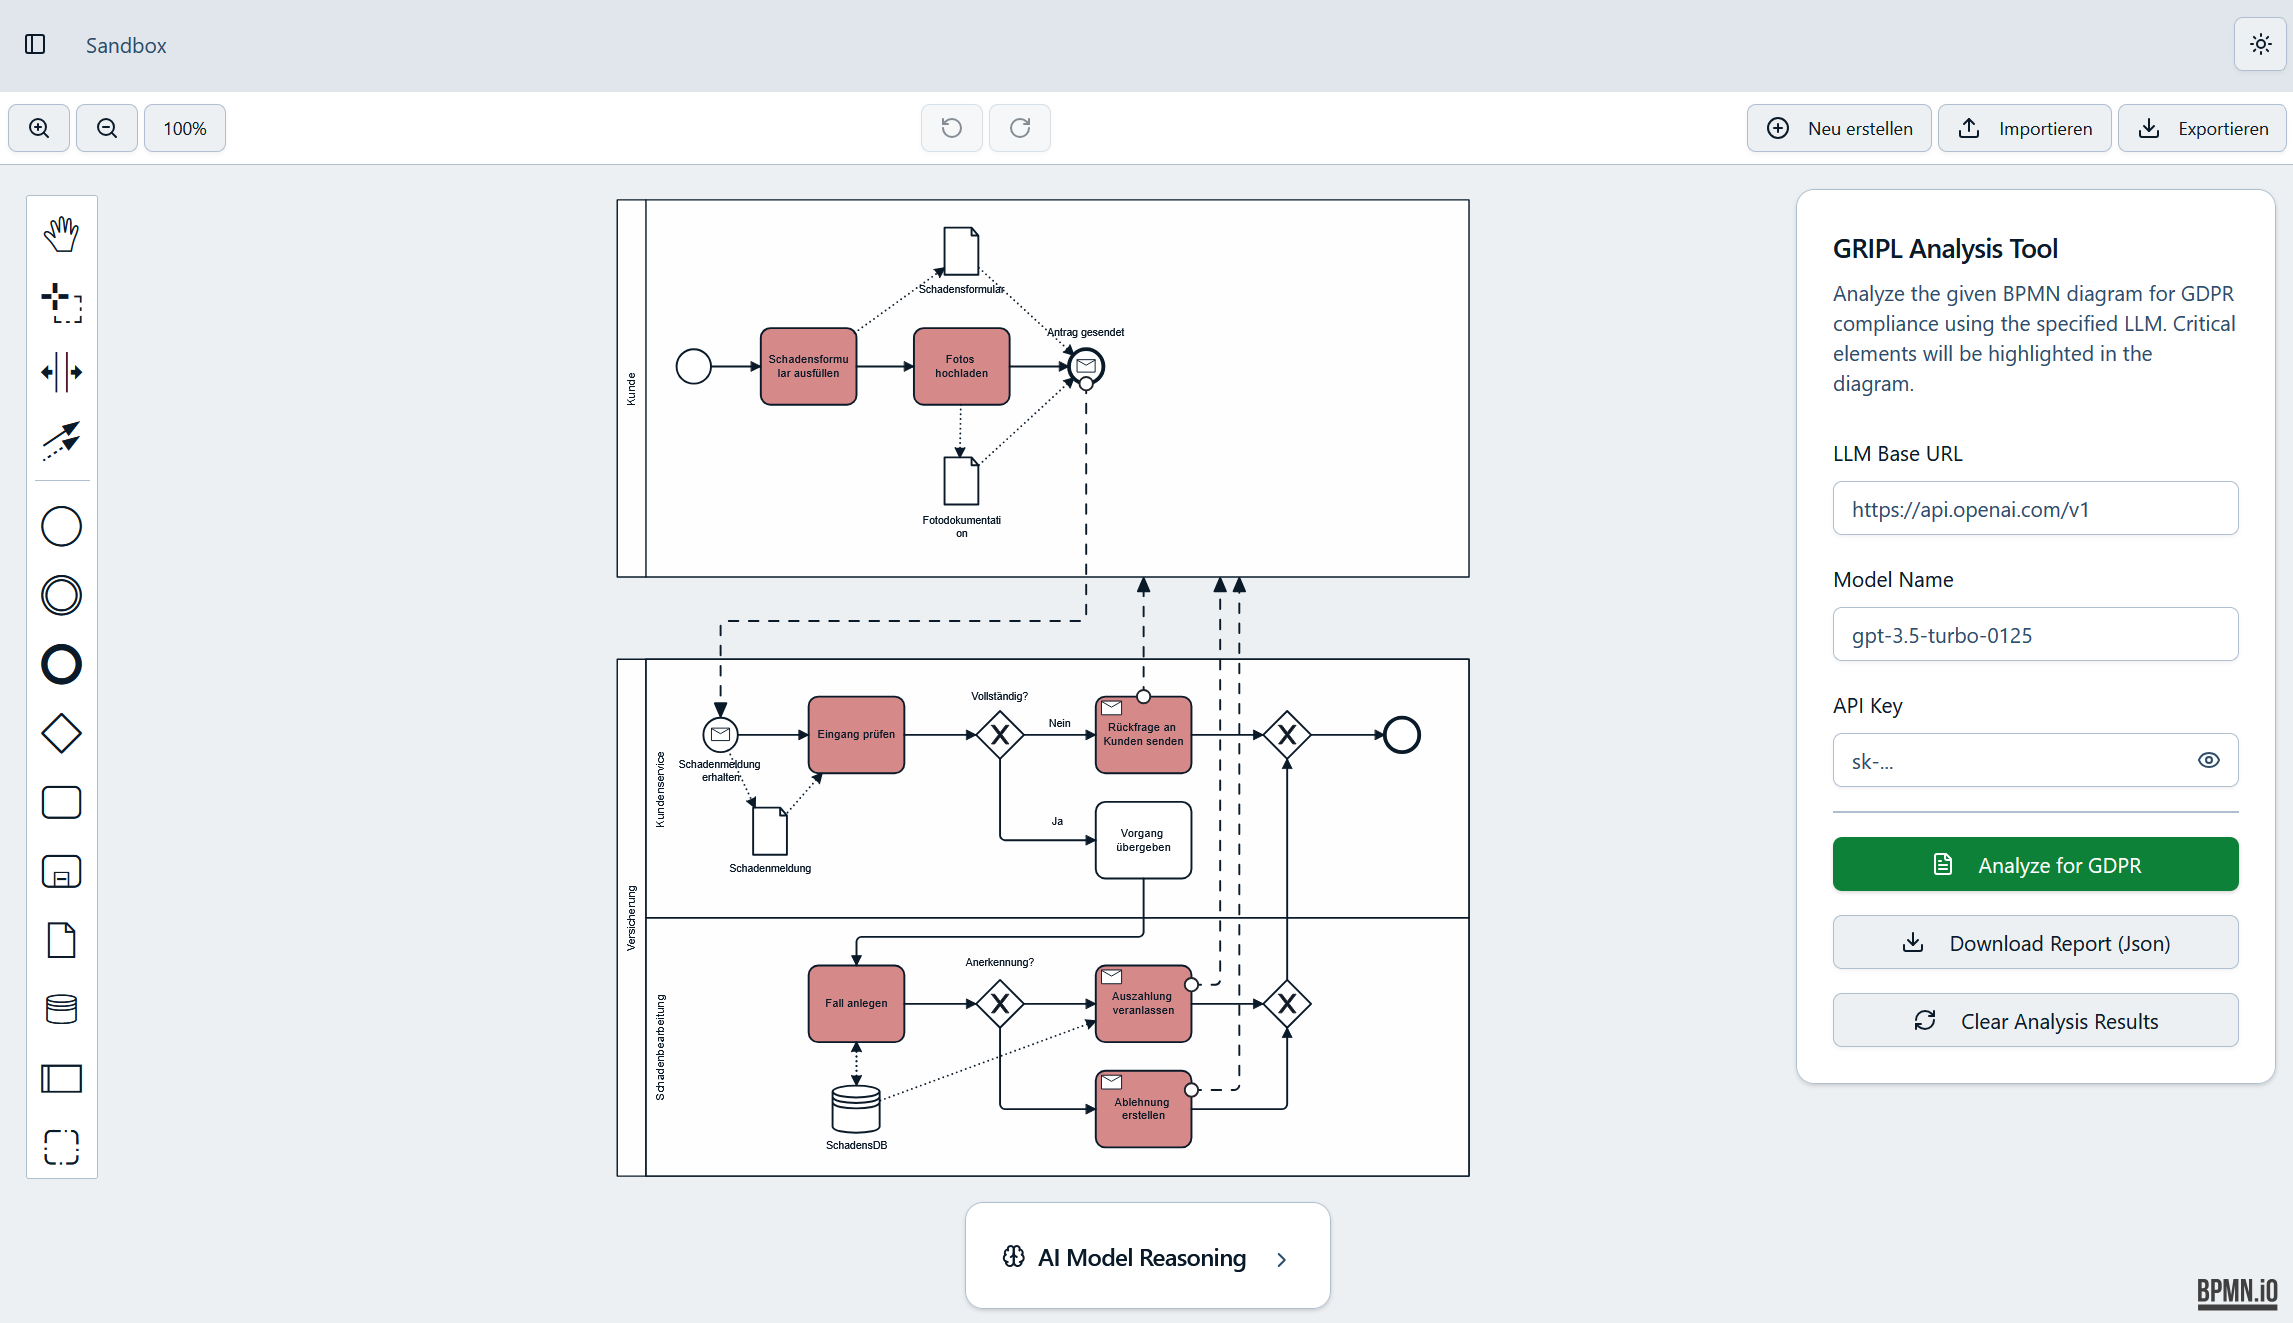
\includegraphics[width=\linewidth]{images/sandbox/sandbox-analyzed-model}
    \caption{Sandbox im Frontend mit hervorgehobenen kritischen Aktivitäten nach Analyse.}
    \label{fig:sandbox-frontend-analyzed-model}
\end{figure}

Außerdem können die vom \ac{LLM} generierten Begründungen zu jeder als kritisch erkannten Aktivität im Editor eingesehen werden. Diese Erläuterungen werden gesammelt in einer aufklappbaren Karte im unteren Bereich des Editors angezeigt, siehe Abbildung \ref{fig:sandbox-frontend-ai-reasoning}.

\begin{figure}
    \centering
    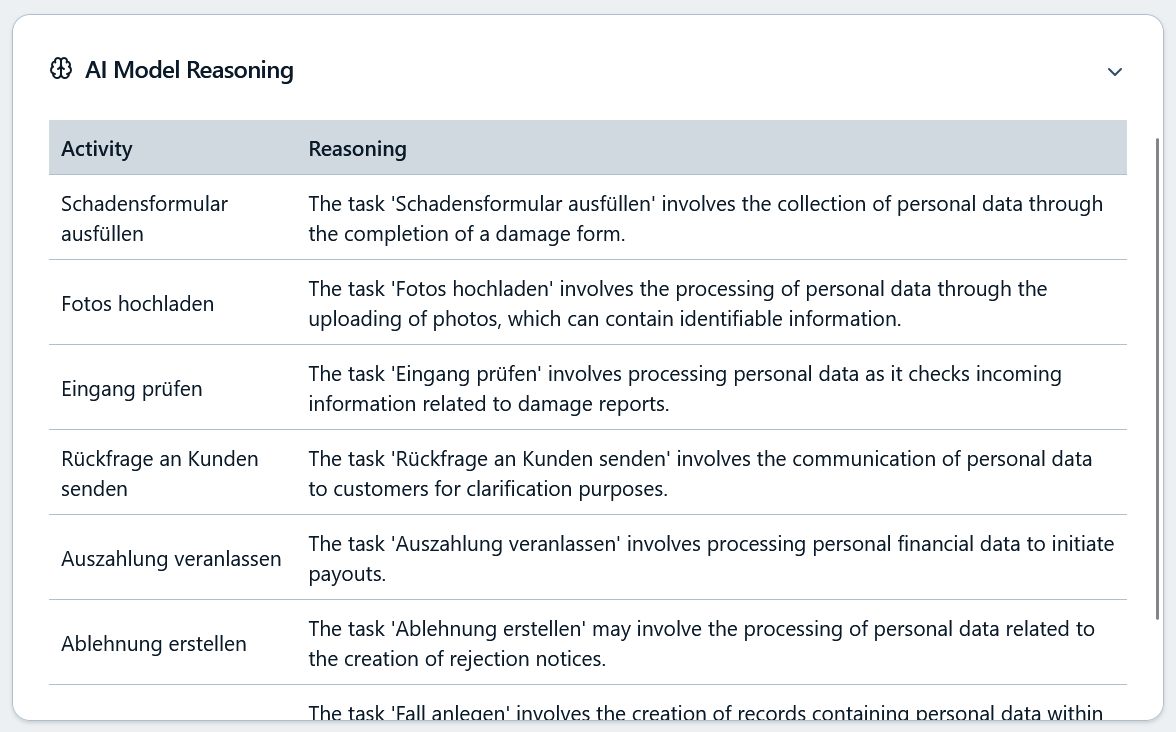
\includegraphics[width=\linewidth]{images/sandbox/sandbox-ai-reasoning}
    \caption{Begründung der Klassifikation durch das LLM in der Sandbox.}
    \label{fig:sandbox-frontend-ai-reasoning}
\end{figure}

Um verschiedene \acp{LLM} vergleichen zu können, verfügt die Sandbox auf der rechten Seite über ein Einstellungsmenü mit konfigurierbaren \ac{LLM}-Parametern (siehe Abbildung \ref{fig:sandbox-frontend-analyzed-model}). Diese Parameter sind identisch zu den in Kapitel \ref{sec:api-design} beschriebenen \texttt{llmProps} und werden beim Starten der Analyse in die API-Anfrage überführt.
\section{Erweiterbarkeit}\label{sec:erweiterbarkeit}

\begin{itemize}
    \item Neue Modelle können über Konfiguration ergänzt werden (Endpunkt, Modellname, API Key)
    \item Neue Klassifizierungsalgorithmen/pipelines können ergänzt werden, wenn sie das vorgegebene HTTP-Schnittstelle unterstützen
    \item Die Testdatensätze werden aus Datenbank ausgelesen und können für jeden Evaluations-Run neu gesetzt werden
\end{itemize}